\documentclass[a4paper,11pt,oneside]{article}
\usepackage[utf8]{inputenc}
\usepackage[a4paper,top=3cm,bottom=3cm,left=3cm,right=3cm]{geometry}
\renewcommand{\familydefault}{\sfdefault}
\usepackage{helvet}
\usepackage[english]{babel}     %% typographie française
\usepackage[style=numeric,language=english,backend=bibtex]{biblatex}
\usepackage{parskip}		%% blank lines between paragraphs, no indent
\usepackage[margin=1cm]{caption}%% give long captions a margin
\usepackage{booktabs}           %% typesetting nice tables
\usepackage{subfig}
\usepackage[pdftex]{graphicx}	%% include graphics, preferrably pdf
\usepackage{pdfpages}
\usepackage[pdftex]{hyperref}	%% many PDF options can be set here
\usepackage{algorithm}
\usepackage{arevmath}     % For math symbols
\usepackage{amsmath}
\usepackage{array}
\usepackage{enumitem}
\usepackage[noend]{algpseudocode}
\pdfadjustspacing=1		%% force LaTeX-like character spacing
\newcolumntype{L}{>{\centering\arraybackslash}m{3.15cm}}

\newcommand{\mylastname}{Adhikari}
\newcommand{\myfirstname}{Ashray}
\newcommand{\mynumber}{30002167}
\newcommand{\myname}{\myfirstname{} \mylastname{}}
\newcommand{\mytitle}{Underwater Image Enhancement}
\newcommand{\mysupervisor}{Prof. Andreas Birk}

\hypersetup{
  pdfauthor = {\myname},
  pdftitle = {\mytitle},
  pdfkeywords = {},
  colorlinks = {true},
  linkcolor = {blue}
}

\addbibresource{references.bib}

\begin{document}
  \pagenumbering{roman}

  \thispagestyle{empty}

  \begin{flushright}
    
\includegraphics[scale=0.8]{bsc-logo}
  \end{flushright}
  \vspace*{40mm}
  \begin{center}
    \huge
    \textbf{\mytitle}
  \end{center}
  \vspace*{4mm}
  \begin{center}
   \Large by
  \end{center}
  \vspace*{4mm}
  \begin{center}
    \LARGE
    \textbf{\myname}
  \end{center}
  \vspace*{20mm}
  \begin{center}
    \Large
    Bachelor Thesis in Computer Science
  \end{center}
  \vfill
  \begin{flushleft}
    \large
    Submission: \today \hfill Supervisor: \mysupervisor \\
    \rule{\textwidth}{1pt}
  \end{flushleft}
  \begin{center}
    Jacobs University Bremen $|$ Department of Computer Science and Electrical Engineering
  \end{center}

  \newpage
  \thispagestyle{empty}

%\subsection*{English: Declaration of Authorship}
 %
  %I hereby declare that the thesis submitted was created and written
  %solely by myself without any external support. Any sources, direct
  %or indirect, are marked as such. I am aware of the fact that the
  %contents of the thesis in digital form may be revised with regard to
  %usage of unauthorized aid as well as whether the whole or parts of
  %it may be identified as plagiarism. I do agree my work to be entered
  %into a database for it to be compared with existing sources, where
  %it will remain in order to enable further comparisons with future
  %theses. This does not grant any rights of reproduction and usage,
 % however.
%
  %This document was neither presented to any other examination board
  %nor has it been published.
%
  %\subsection*{German: Erklärung der Autorenschaft (Urheberschaft)}
 %
  %Ich erkläre hiermit, dass die vorliegende Arbeit ohne fremde Hilfe
  %ausschließlich von mir erstellt und geschrieben worden ist. Jedwede
  %verwendeten Quellen, direkter oder indirekter Art, sind als solche
  %kenntlich gemacht worden. Mir ist die Tatsache bewusst, dass der
  %Inhalt der Thesis in digitaler Form geprüft werden kann im Hinblick
  %darauf, ob es sich ganz oder in Teilen um ein Plagiat handelt. Ich
  %bin damit einverstanden, dass meine Arbeit in einer Datenbank
  %eingegeben werden kann, um mit bereits bestehenden Quellen
  %verglichen zu werden und dort auch verbleibt, um mit zukünftigen
  %Arbeiten verglichen werden zu können. Dies berechtigt jedoch nicht
  %zur Verwendung oder Vervielfältigung.
%
  %Diese Arbeit wurde noch keiner anderen Prüfungsbehörde vorgelegt
  %noch wurde sie bisher veröffentlicht.

  %\vspace{20mm}
	%12.05.2021, 
\includegraphics[scale=0.04]{signature.jpg}\\
  %Date, Signature
  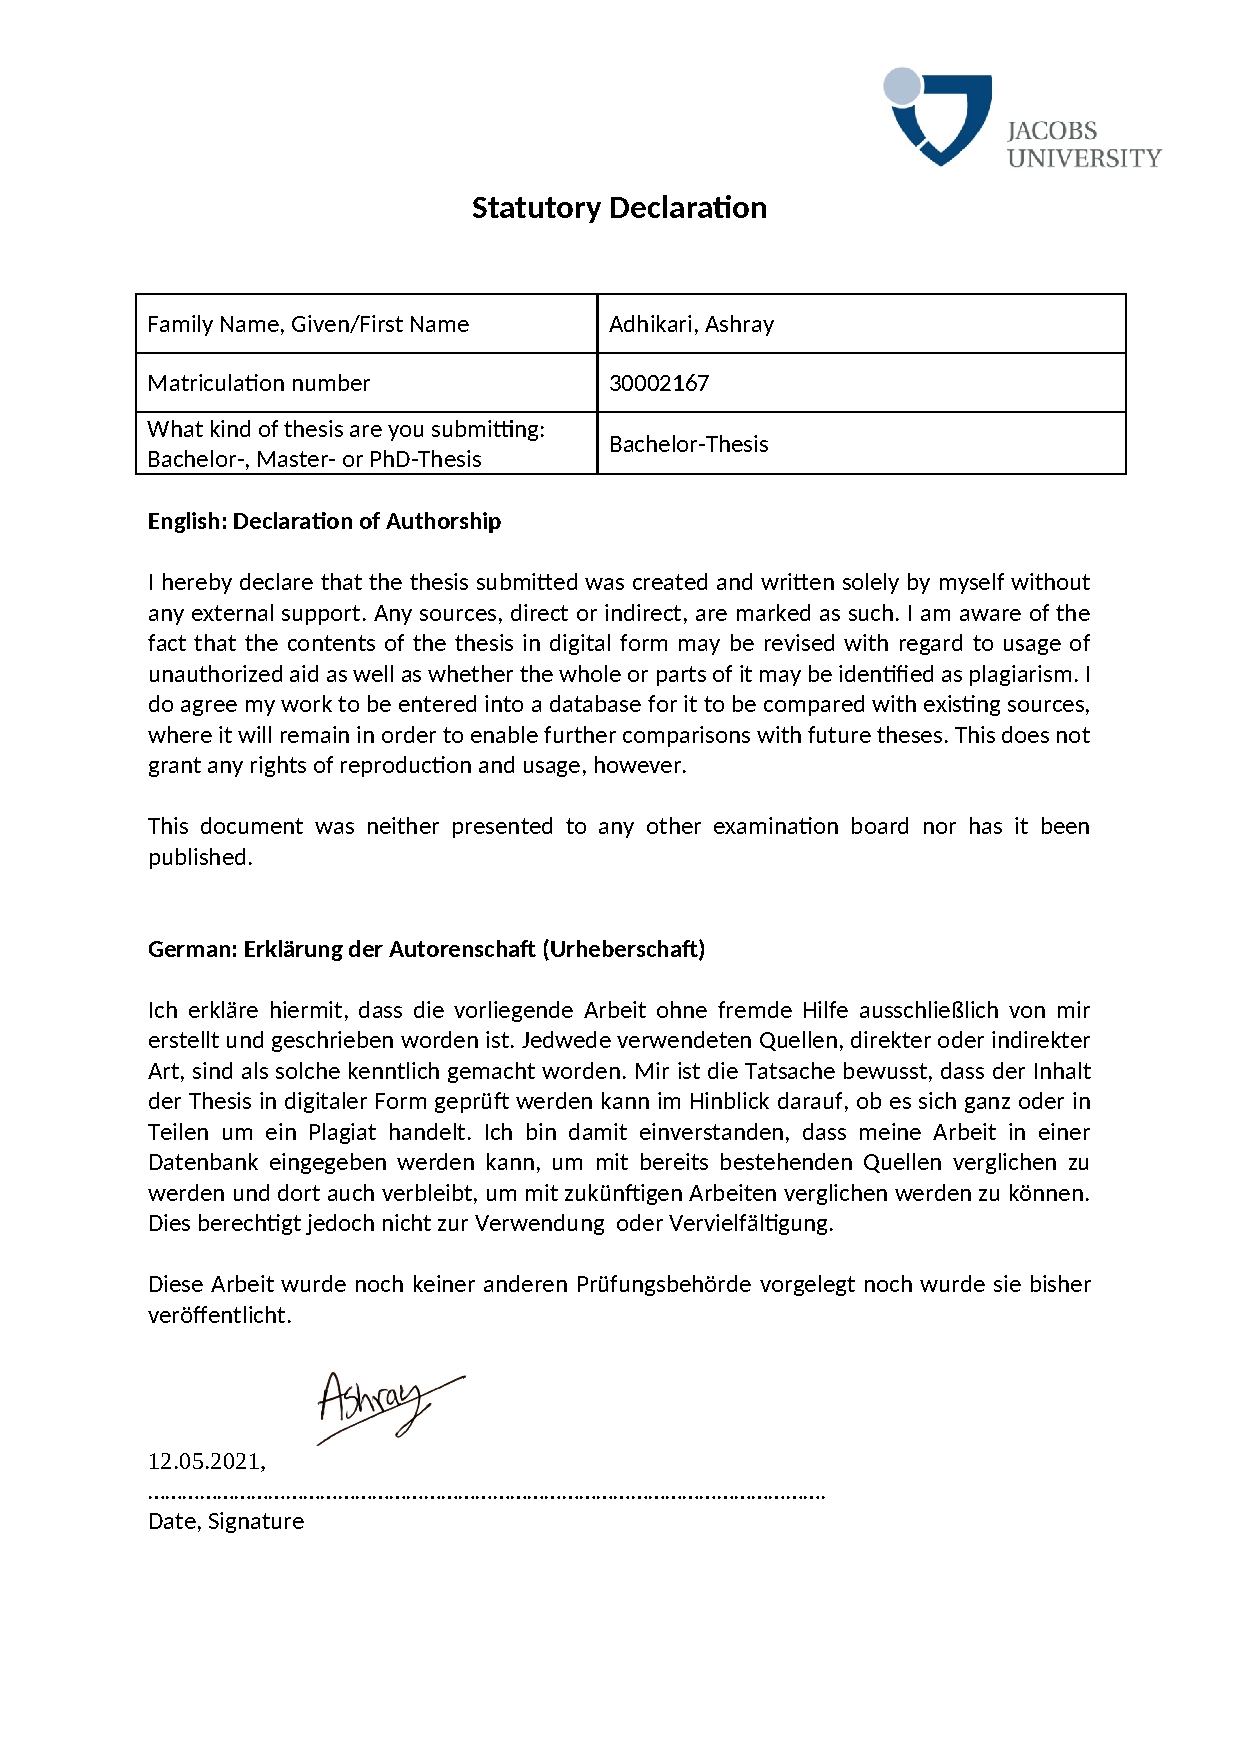
\includepdf[pages=-]{Declaration.pdf}
  % \begin{center}
  %   \Large \textbf{Statutory Declaration}
  %   \vspace*{8mm}
  % \end{center}

  % \begin{center}
  %   \begin{tabular}{|l|p{85mm}|}
  %     \hline
  %     Family Name, Given/First Name & \mylastname, \myfirstname \\
  %     Matriculation number & \mynumber \\
  %     Kind of thesis submitted & Bachelor-Thesis \\
  %     \hline
  %   \end{tabular}
  %   \vspace*{8mm}
  % \end{center}

  % \subsection*{English: Declaration of Authorship}
 
  % I hereby declare that the thesis submitted was created and written
  % solely by myself without any external support. Any sources, direct
  % or indirect, are marked as such. I am aware of the fact that the
  % contents of the thesis in digital form may be revised with regard to
  % usage of unauthorized aid as well as whether the whole or parts of
  % it may be identified as plagiarism. I do agree my work to be entered
  % into a database for it to be compared with existing sources, where
  % it will remain in order to enable further comparisons with future
  % theses. This does not grant any rights of reproduction and usage,
  % however.

  % This document was neither presented to any other examination board
  % nor has it been published.

  % \subsection*{German: Erklärung der Autorenschaft (Urheberschaft)}
 
  % Ich erkläre hiermit, dass die vorliegende Arbeit ohne fremde Hilfe
  % ausschließlich von mir erstellt und geschrieben worden ist. Jedwede
  % verwendeten Quellen, direkter oder indirekter Art, sind als solche
  % kenntlich gemacht worden. Mir ist die Tatsache bewusst, dass der
  % Inhalt der Thesis in digitaler Form geprüft werden kann im Hinblick
  % darauf, ob es sich ganz oder in Teilen um ein Plagiat handelt. Ich
  % bin damit einverstanden, dass meine Arbeit in einer Datenbank
  % eingegeben werden kann, um mit bereits bestehenden Quellen
  % verglichen zu werden und dort auch verbleibt, um mit zukünftigen
  % Arbeiten verglichen werden zu können. Dies berechtigt jedoch nicht
  % zur Verwendung oder Vervielfältigung.

  % Diese Arbeit wurde noch keiner anderen Prüfungsbehörde vorgelegt
  % noch wurde sie bisher veröffentlicht.

  % \vspace{18mm}

	% 12.05.2021, 
\includegraphics[scale=0.04]{signature.jpg}\\
  % \dotfill\\
  % Date, Signature

\newpage

  \section*{Abstract}
  
  %Consider this a separate document, although it is submitted together
  %with the rest. The abstract aims at another audience than the rest
  %of the proposal. It is directed at the final decision maker or
  %generalist, who typically is not an expert at all in your field, but
  %more a manager kind of person. Thus, don't go into any technical
  %description in the abstract, but use it to motivate the work and to
  %highlight the importance of your project.

  %(target size: 15-20 lines)
  Underwater imaging plays a vital role in Underwater exploration and scientific research. However, most Underwater images suffer from severe degradation due to light scattering and absorption. This paper compares different Underwater image enhancement methods and selects the most suitable enhancement methods for images extracted from the Underwater video from the Valentine memorial bunker:
  \begin{enumerate}
  \item
  We introduce the fundamental problems in Underwater imaging.
  \item
  We review different underwater enhancement methods and select four enhancement methods that help enhance our Underwater images.
  \item
  We use both the visual and quantitative analysis of the enhanced Underwater images to compare the enhancement methods.
  \end{enumerate}
  For the quantitative analysis, we use the non-reference quality metric to compare the enhanced Underwater Images. Our comparison of the enhancement methods attempts to provide the most suitable Underwater enhancement method for our images.
  \newpage
  \tableofcontents

  \clearpage
  \pagenumbering{arabic}

  \section{Introduction}

  %This, like the rest, addresses fellow experts from your field (but
  %not from your particular topic of research). Here you should
  %technically connect to the main concepts from that field and give an
  %outline of your project, stating the research/engineering question
  %that you want to get answered by your project.

  %(target size: 1-2 pages)
  
  Researchers today strive to capture high-quality underwater images for various Underwater activities \cite{15} but, Underwater imaging is a challenging field in computer vision research instead of land photography. Many physical and chemical characteristics of Underwater conditions raise issues that we can easily overcome in land photography \cite{15}.\\
  \\
  Underwater imaging raises new challenges and problems due to the absorption and scattering effects of light underwater, which generates low-contrast images and causes distant objects to appear blurry and misty \cite{3}. As light moves from air to water, it is partly reflected, and the amount of light entering reduces as we start going deeper. So, Underwater images appear dark as depth increases and the colors drop off one by one depending on the wavelength \cite{4}. Due to the varying degrees of attenuation encountered by the light traveling in water with different wavelengths, the ambient underwater environment is dominated by a bluish tone \cite{20}.\\
  The light received by the camera is mainly generated by a direct component that reflects light from the object, forward scattering that randomly deviates light on its way to the camera, and the backscattering component that reflects light toward the camera before the light reaches the objects \cite{21}. In an underwater scene, light accepted through a camera can be represented as a linear superposition of all three components.  So, forward scattering causes the blurring on the image, and the backscattering masks the details of the scene \cite{21}.\\
  \\
  Besides the absorption and scattering effects of light by the water, water quality also influences the quality of underwater images. The presence of suspended particles with significant size and density in the medium also causes light to be scattered and absorbed \cite{8}. Haze is caused by the suspended particles such as sand, minerals, and plankton in the water body. Some portion of the light meets these suspended particles as light reflected from the object propagates towards the camera \cite{13}.\\
  \\
  Due to certain challenging underwater conditions, traditional enhancing techniques appear to be strongly limited for Underwater Images. Traditional image restoration methods use an atmospheric scattering model to restore underwater images\cite{11}, and underwater conditions are considered similar to dense fog on land. Still, unlike fog, underwater illumination is spectrally deprived as water attenuates different wavelengths of light to different degrees \cite{2}. Applying conventional color correction methods designed for terrestrial environments on Underwater images will lead to undesired artifacts since the red component of the Underwater image is much weaker than the green and blue components \cite{6}.\\
  \\
In this document, we test and perform a qualitative and quantitative comparison of different Underwater enhancement methods on the images extracted from Underwater videos of the Valentine memorial. The rest of the document is structured as follows. Section \hyperref[sec:2]{2} discusses the related work done in Underwater Image Enhancement. Section \hyperref[sec:3]{3} discusses our method to enhance and compare the images and describes the enhancements methods in detail. Section \hyperref[sec:4]{4} showcases the results and analysis of the experiment on the extracted images. Section \hyperref[sec:5]{5} provides the conclusion of the document.  

  \section{Discussion of Related Work}
  \label{sec:2}

  %This part should make clear which question, exactly, you are
  %pursuing, and why your project is relevant/interesting. This is the
  %place to explain the background and to review the existing
  %literature. Where does your project extend the state of the art?
  %What weaknesses in known approaches do you hope to overcome? If you
  %have carried out preliminary experiments, describe them here.

  %(target size: 5-10 pages)
  Over the years, several methods have been specifically designed according to the characteristics of underwater images, e.g., hazing, color casts, and low contrast \cite{15}. This section will discuss different physics-based, color correction, haze removal, fusion-based, and CNN-based Underwater Image Enhancements and Restoration methods.\\
  \\
  In a Physics-based approach for recovery of visibility in Underwater scenes, raw images are taken through different stages of a polarizing filter. In 2004 Schechner and Kerpel \cite{19} proposed a physics-based approach that "inverts the image formation process to recover a good visibility image of the object" \cite{19}. The algorithm presented were based on photos taken through a polarizer at different orientations \cite{19}. The physics-based methods require high computing resources and long execution time, and the polarizer used in the approach is expensive \cite{8}. We will not consider the physics-based method for our analysis.\\
  \\
  In recent years many studies have proved the effectiveness of deep-learning methods for various computer vision tasks. But, very few of them have been effective in underwater image enhancement. In 2017, Perez et al. \cite{22} proposed a "CNN-based Underwater Image Enhancement method that uses a convolution neural network to learn the transformation from raw acquired images to enhanced images using a pair of degraded and recovered underwater photos" \cite{22} \cite{15}. Then in 2018, Li et al. \cite{23} proposed WaterGAN, "a generative adversarial network for generating synthetic realistic underwater images from in-air image and depth maps" \cite{23}. He used the raw Underwater, actual color-in air, and the depth data to feed a deep learning network for correcting color casts in underwater images \cite{15}. Finally, to relax the need for paired underwater images for network training and allow the use of unknown underwater images, Li et al. \cite{7} proposed an "Underwater Image Correction model based on a Weakly Supervised Color Transfer" \cite{15}. In this method, a color correction algorithm is applied to correct the color cast and produce a natural appearance of the sub-sea image. Then a pair of dictionaries based on sparse representation are used to sharpen the image and enhance the details \cite{7}. Thus, the Deep Learning-based Underwater Enhancement methods have, to some extent, proven to be effective in enhancing underwater images. But due to the lack of data required to train the model, we will not use the CNN-based model to enhance the extracted images from the Valentine memorial.
\\
  \\
    Classic Retinex theory assumes that the images can be decomposed into two components, reflectance and illumination. The classic Retinex model is not suited for the low-light image enhancement problem, as intensive noise exists in low-light images \cite{5}. In 2018 Li et al. \cite{5} proposed a "Structural Revealing Image Enhancement Algorithm Using a Robust Retinex Model" \cite{5}. This method proposed a Robust Retinex, which additionally considers a noise map compared to the conventional Retinex model to improve the performance of enhancing low-light images accompanied by intense noise \cite{5}. Even though this method was not made for underwater conditions, it can be generalized to handle Underwater Image Enhancements \cite{5}.\\
  In 2019 B. Gao et al. \cite{6} proposed an "Underwater Image Enhancement model inspired by the morphology and function of the teleost fish retina to solve the blurring and the non-uniform color biasing problem of underwater images" \cite{6}. The motivation behind this approach is that the visual system of the oceanic creatures has evolved to adapt to the natural statistics of aquatic scenes \cite{6}. So, modeling the perception and imaging mechanisms of the oceanic creatures will give us new insights into processing Underwater images \cite{6}.\\
  \\
   Wavelet decomposition algorithm decomposes an original image into a sequence of new images of decreasing size \cite{24}. In a fusion-based approach, weight maps are computed and fused to enhance the image \cite{10}.  In 2016 A. Khan et al. \cite{9} proposed a "wavelet-based fusion method to enhance hazy underwater images by addressing low contrast and color attenuation issues" \cite{9}. Two input images are generated from the hazy image by color correction using histogram stretching and contrast enhancement using contrast limited adaptive histogram equalization (CLAHE) \cite{9}. Both input images are decomposed into wavelet coefficients, and the coefficient is fused using an algorithm that eliminates unwanted low and high frequency present in the image \cite{9}. Finally, the inverse composition is applied to the fused coefficient to get a synthesized enhanced image. \cite{9}\\
  In 2017 Wang et al. \cite{12} proposed a different "fusion-based model applied to a frequency domain" \cite{12}. It involves two inputs represented as color corrected and contrast-enhanced images extracted from the original image \cite{12}. First, the input images are decomposed into low frequency and high-frequency components using a three-scale wavelet operator \cite{12}. Then, Multi-scale fusion principles are applied to the low and high-frequency components \cite{12}. The fusion principle for low-frequency components involves a weighted average of the components, and the high-frequency component involves the local variance of components \cite{12}. Finally, the fused image is obtained by reconstructing the new fused low frequency and high-frequency components \cite{12}.\\
  \\
  As the weight maps computed in a fusion-based approach may introduce artifacts in the image, P. Honnutagi et al. in 2018 \cite{10} proposed a method to overcome this problem by using an "optimized fusion method of weight maps, where multi-step fusion is used to perform a fusion of weight maps computed from illumination estimation and contrast-enhanced inputs of the original image" \cite{10}. First illumination estimation is applied on the image to improve visibility, then contrast limited adaptive histogram equalization (CLAHE) is used to derive the second input, which improves the contrast of the image \cite{10}. Next, saliency, luminance, and chromatic weight maps are computed for each derived inputs \cite{10}. After computing each weight map, the final weight map is produced by multiplying all three weight maps \cite{10}. Finally, an enhanced image is generated from the multi-step fusion technique by using the Gaussian and mean operators on both weight maps \cite{10}.\\
  \\
  The Dark Channel Prior method is based on the observation that in a clear day image, there exists some pixels which have a very low intensity in at least one color channel \cite{15}. Due to the similarity between hazed outdoor images and underwater images, the Dark Channel-based hazing method is used for underwater image enhancement. Chao and Wang in 2010 \cite{25} used the "Dark Channel Prior method directly to enhance the clarity of the image" \cite{25}. Using dark channel prior depth of the Underwater Image is estimated, but this method does not solve the problem of absorption \cite{25}.\\
 In 2011 Yang et al. \cite{8} proposed a "DCP-based fast Underwater Image Enhancement method that can effectively enhance Underwater Image and reduce execution time" \cite{8} This method used a median filter instead of a soft matting procedure to estimate the depth map of the image \cite{8}. The Dark Channel Prior is calculated to estimate air-light, and the depth map is generated using a median filter \cite{8}. A color correction method is employed to enhance the color contrast of the image.\cite{8}\\
  \\
  As enormous scene depth causes more object blurriness in Underwater images, Y. Peng et al. in 2015 \cite{3} proposed a method that "measures scene depth from image blurriness to estimate depth map for Underwater Image enhancement" \cite{3}. The method is based on the observation that objects farther from the camera are more blurry for Underwater Images \cite{3}. To overcome the limitation of DCP, the depth estimation method calculates the difference between the original and the multi-scale Gaussian filter to estimate the pixel blurriness map \cite{3}. Then, by assuming that the depth in the small local patch is uniform, the max filter is applied to the pixel blurriness map \cite{3}. Finally, closing by morphological reconstruction (CMR) and the guided filter are used to refine the depth map \cite{3}.\\
   Most existing methods based on the DCP method convert information from three RGB channels to one dark channel. Still, those methods are inadequate in cases where chromatic information is essential for restoration \cite{17}. Zhou et al. in 2019 \cite{17} proposed a "method to handle the scattering and absorption problems of light with different wavelengths base on the color-line model" \cite{17}. The color line is a regularity in images, which shows that the pixel values of small patches are distributed along a  one-dimensional line in the RGB space \cite{17}. First, the image patches that exhibit the characteristics of the color-line prior are filtered out, and the color line of the patches are recovered \cite{17}. "Then, the local transmission for each patch is estimated based on the offsets of the color lines along the background-light vector from the origin" \cite{17}. In order to solve the non-linear optimization problem for transmission in an Underwater environment, Zhou et al. also presented an alternating iterative algorithm \cite{17}. Finally, using Wavelength Compensation, color restoration of the Underwater Image is performed \cite{17}.\\
  \\
  The transmission map is reducing exponentially with scene depth, which is difficult to estimate in Underwater Environment. So, Mi et al. in 2018 \cite{11} proposed an "enhancement method using a multi-scale gradient-domain contrast enhancement strategy to increase visibility and compensate the attenuation of color saturation according to the estimated transmission" \cite{11}. Before applying the enhancement method, first, the Underwater Image is white-balanced to remove the color casts while producing a natural appearance of the Underwater image \cite{11}. Then, to prevent halo artifacts, a multi-scale gradient enhancement strategy is used \cite{11}. Finally, by compensating color saturation according to the estimated transmission, we get the enhanced image \cite{11}.\\ 
  \\
  Several other methods have been proposed to remove the haze and increase the contrast of Underwater images. For example, Ancutti et al. in 2018 \cite{16} proposed a method that uses "color balance and fusion methods to enhance Underwater Images" \cite{16}. First, the White Balanced version of the original image is decomposed into two input images to enhance the color contrast and edge sharpness \cite{16}. Then, the weight maps are defined to preserve the qualities and reject the defaults of the inputs \cite{16}. Finally, the multi-scale fusion method decomposes the image into a sum of bandpass images \cite{16}. The method is motivated by the human visual system, which is very sensitive to sharp transition appearing in smooth image \cite{16}.\\
  \\
  Since most Underwater dehazing methods are for still underwater images, Emberton et al. \cite{2} in 2018 proposed a "dehazing method that improves visibility in images and videos by detecting and segmenting image regions; that contain only water" \cite{2}. First, the spectral distortion problem is addressed by automatically selecting the most appropriate white balancing method based on the most dominant color of the water \cite{2}. Second, varying patch sizes are used to estimate light scattered from underwater particles into the line of sight of the camera \cite{2}. Third, entropy-based segmentation is used to localize pure haze region that informs the features to select for the scattered light \cite{2}. Finally, image-specific transmission value is allocated to pure haze regions to avoid generating artifacts \cite{2}.\\
  \\
   The presence of an artificial light source in Underwater Image increases the scattering of light Underwater. So, Chiang and Chen in 2012 \cite{13} proposed a method to "enhance underwater images by dehazing algorithm to compensate the attenuation difference along the propagation path, and to take the influence of the possible presence of an artificial light source into consideration" \cite{13}. Dark channel prior is first used to estimate the distances of scene objects to the camera \cite{13}. Based on the depth map, the foreground and background areas within the image are segmented \cite{13}. The light intensity of the foreground and background are compared to determine whether artificial is used \cite{13}. Dehazing algorithm and wavelength compensation are used to remove the haze effect and color change along the Underwater propagation path to the camera \cite{13}.\\
  \\
  Histogram equalization involves transferring the histogram of an original image to an evenly distributed form \cite{1}. For an Underwater image histogram equalization method is mainly used for color correction of the degraded image. Beilei Hu et al. \cite{1} in 2013 proposed a method that uses "inhomogeneous illumination to get a clearer image, and then processes it to use color image histogram equalization to get more color information which gives out true color correction" \cite{1} Inhomogeneous intensity can compensate for the loss of light intensity due to light attenuation and decrease backscattering effect caused by the scattering of Underwater light \cite{1}. As the light in Underwater is heavily attenuated, if the light source is not strong enough, the intensity of the target object in the image is fragile \cite{1}. So, it is necessary to use inhomogeneous illumination as the light source \cite{1}. During color histogram equalization, each channel of the image is histogram equalized by monotonically increasing grey level transform \cite{1}. These images of different color channels combined to form a high contrast image \cite{1}.\\
  \\
   Underwater Images are used for many different computer vision applications, and different kinds of images are required. So, Li et al. in 2016 \cite{21} proposed an "Underwater Enhancement algorithm, which includes both image dehazing and contrast enhancement algorithm that is built on minimum information loss principle to restore the visibility, color, and natural appearance of Underwater images" \cite{21}. Two different output images are produced for applications using this method \cite{21}. The first version with relatively natural color and natural appearance is suitable for displaying the image, and the second version with high contrast and brightness is used for extracting more valuable information and revealing more details \cite{21}. For the image dehazing algorithm, the global background light is first estimated using a hierarchical searching technique based on quad-tree subdivision followed by removing suspended particles using the dark channel prior algorithm \cite{21}. The disturbance of bright objects is removed, and the global background light is determined according to the properties of light traveling in water \cite{21}. Then, to minimize information loss, the medium transmission map of the color channels is defined \cite{21}. Underwater images with high contrast and brightness play a vital role in object detection, classification, etc. \cite{21}. The contrast enhancement algorithm proposed in this method is based on the histogram distribution of visually appealing natural-scene images \cite{21}. The histogram distribution prior is counted for five natural-scene image datasets \cite{21}. Then, the average histogram distributions of natural scenes are regarded as a template and are followed by the approximate histogram matching to adjust the histogram distributions of haze-free underwater images obtained by the dehazing algorithm \cite{21}.\\
  \\
  Most Underwater images are degraded by light absorption and scattering, which causes a single color to dominate the image. Iqbal et al. in 2007 \cite{4} proposed a method based on "slide stretching". First, contrast stretching of the RGB algorithm is used to equalize color contrast in the image \cite{4}. Then, the RGB image is transformed into HSI color space, using the saturation and intensity transfer function to increase the actual color and brightness of Underwater images \cite{4}. Using two side stretching models helps equalize the color contrast in images and address lighting \cite{4}.
 \newpage
  \section{Methodology}
  \label{sec:3}
  %This is the technical core of the thesis. Here you lay out your how
  %you answered your research question, you specify your design of
  %experiments or simulations, point out difficulties that you
  %encountered, etc.
  %
  %(target size: 5-10 pages)
  In the previous section, we saw varieties of Underwater image enhancement methods that strive to solve different problems raised by Underwater imaging. While almost all those methods may solve various issues raised by Underwater imaging, we will not test and use all those methods due to the lack of data or information about our Underwater Scene. So, we have selected \cite{4}, \cite{8}, \cite{26} and \cite{16} methods to test and compare the result for our Underwater image extracted from the Underwater videos of the Valentine memorial. These methods help solve some of the common problems in Underwater imaging, which gives us information on which plan would be best suited for our Underwater images. Furthermore, we use the An "Underwater Color Image Quality Evaluation Metric(UCIQE)" \cite{18} and "Underwater Image Quality Measure(UIQM)" \cite{29} for the quantitative comparison of the enhancement methods.\\
  \\
  \begin{figure}[H]
  \begin{center}
    \subfloat[]{\includegraphics[width=0.5\linewidth]{../Underwater-Image-Enhancements/InputImages/Valentine_196.png}}
    \subfloat[]{\includegraphics[width=0.5\linewidth]{../Underwater-Image-Enhancements/InputImages/Valentine_60.png}} \\
    \subfloat[]{\includegraphics[width=0.5\linewidth]{../Underwater-Image-Enhancements/InputImages/Valentine_129.png}}
    \subfloat[]{\includegraphics[width=0.5\linewidth]{../Underwater-Image-Enhancements/InputImages/Valentine_10.png}}
  \end{center}
  \caption{Original Degraded images}
  \label{fig:1}
\end{figure}
  Before applying the enhancement algorithms, we extract the image from the Underwater videos of the memorial submarine bunker Valentine. From those extracted images, we select a specific sequence of images to use for our enhancement algorithm. For the selected sequence of images we crop out the regions with the timestamps and texts as it interfers with the enhancement methods. Now, if we look at our images in Fig \ref{fig:1}, we can see that the quality of the Underwater image is affected by different Underwater image characteristics. The Underwater image has low color contrast and has a severe blurring effect. So, we use the selected Underwater enhancement methods to enhance and compare the output images.\\
  First, we need to learn about these Underwater enhancement methods and the problems these methods are trying to solve.
  \subsection{Underwater Image Enhancement using an Integrated Color Method \cite{4}}
  As discussed above Integrated Color Method is based on slide stretching. In this method, we use the HSI(Hue, Saturation, or Intensity) color model, as it provides a more comprehensive color range by controlling the color elements of the image \cite{4}. For instance, the 'S' and 'I' value controls the blue color element in the image to create a range from pale blue to deep blue. We can use this color model to control the contrast ratio in Underwater Images by increasing or decreasing the value \cite{4}.\\
We can express the Integrated Color Model approach using the following algorithm.
  \begin{algorithm}
	\caption*{Underwater Image Enhancement using an Integrated Color Method \cite{4}}
	\begin{algorithmic}

	\Procedure{Enhance}{degraded\_image}
    \State Contrast Stretching Of RGB Image
    \State Transform RGB Images to HSI \Comment{Using Saturation and Intensity transfer function}
    \State Stretch Saturation and Intensity of the HSI image  \Comment{Using the transform function}
    \State Transform Image Back to RGB color space
    \State
    
    \Return enhanced\_image
\EndProcedure

\end{algorithmic}
\end{algorithm}\\
We used a contrast stretching algorithm to enhance the contrast of the Underwater Image. When applying contrast stretching to color images, each color channel is stretched using the same scaling to maintain the correct color ratio. In a Contrast stretching algorithm, a linear scaling function to the pixel value is used. We scale each pixel in the Image using the following equation \cite{4}.
$$P_{o} = (P_{i} - l_c) \times (max_v - l_c)  / (h_c - l_c) + min_v$$
Where \cite{4},
\begin{itemize}
\item
$P_{0}$ is the normalized output pixel value
\item
$P_{i}$ is the input/considered pixel value
\item
$min_v$  minimum value of the output range and since for RGB we are using image value from 0 to 255, $min_v = 0$
\item
$max_v$ maximum value of the output range and since for RGB we are using image value from 0 to 255, $max_v = 255$
\item
$l_c$ is the lowest pixel value currently present in the image
\item
$h_c$ is the highest pixel value currently present in the image 
\end{itemize}
To balance the red and green channel to that of the blue channel first histogram stretching into both sides is performed to get a well-balanced histogram. Using the HSI color model, we can get the true color of the Underwater images using the saturation parameter. The lighting problem in Underwater scenes is solved using the Intensity parameters. \cite{4} \\
\\
This method attempts to solve the lighting problem and extract the underwater images' true colors but mostly fails to enhance the highly deteriorated Underwater images.

\subsection{Low Complexity Underwater Image Enhancement Based on Dark Channel Prior \cite{8}}
Dark Channel Prior (DCP) is a popular classic Image Enhancement method. Most dark channel prior methods use a soft matting algorithm to eliminate the transmission to reconstruct a scene, but this requires heavy computing resources to smooth and optimize the transmission map \cite{8}. So, in this method, we estimated transmission $\tilde{t}(x)$ directly using the median filter, then to improve the color contrast of the object, we use an unsupervised color correction method \cite{8}.\\
We can model the captured image as direct reflection of light from the object and the reflection of particles from the medium. So, the captured image I(x) is defines as \cite{8}:
$$I(x) = J(x)t(x) + A(1-t(x))$$
J(x) is the output scene radiance,t(x) is the transmission map of the medium, and A is the global atmospheric light. Here, the first term is the direct attenuation, and the second term is called the air-light \cite{8}. Then, we can use this equation for the output scene radiance J(x) by rewriting the equation as \cite{8}:
$$J(x) = \frac{(I(x) - A)}{t(x)} + A$$
For the above equation,  we computed the atmospheric light A using the Dark channel prior method. As the dark channel of the hazy image approximates the haze denseness, we can use the dark channel prior to detect the highest haze-opaque region. For, this method we use the top $0.01\%$ of the brightest pixels in the dark channel \cite{8}. Then, among those pixels, we select the pixels with the highest intensity in the observed image as the atmospheric light A \cite{8}.\\
We use the median filter to calculate the estimated transmission map of the input image for this method. We can express the estimated transmission $\tilde{t}(x)$ using the following equation.
$$\tilde{t}(x) = 1 - \min_{c} (\underset{y\in\psi(x)}{median} \frac{I_{c}(y)}{A_{c}})$$
After computing the scene radiance of the image we used the color correction algorithm to achieve a good visual quality image. In Underwater conditions, images are not color balanced correctly as blue color dominates most of the images \cite{8}. So, first we need to calculate the average of each color components \cite{8}. If we assume size of the image is $M \times N$ and the images $I_R, I_G, I_B$ represent the red, green and blue compoents of the image \cite{8}. We can calculate the average of each color channels as \cite{8}:
$$R_{avg} = \frac{\sum_{i=1}^{M} \sum_{j=1}^{N}I_{R}(i,j)}{M \times N}$$
$$G_{avg} = \frac{\sum_{i=1}^{M} \sum_{j=1}^{N}I_{G}(i,j)}{M \times N}$$
$$B_{avg} = \frac{\sum_{i=1}^{M} \sum_{j=1}^{N}I_{B}(i,j)}{M \times N}$$
Since, Underwater images is dominated mostly by blue color, we can use the blue color to balance the red and green colors. So, using the blue color channel, the other two colors are calculated as follows \cite{8}:
$$\tilde{I_R}(i,j) = \frac{B_{avg}}{R_{avg}}I_R(i,j)$$
$$\tilde{I_G}(i,j) = \frac{B_{avg}}{G_{avg}}I_G(i,j)$$
We can summerize the "Low Complexity Underwater Image Enhancement Based on Dark Channel Prior" \cite{8} method using the following algorithm.
\begin{algorithm}
	\caption*{Low Complexity Underwater Image Enhancement Based on Dark Channel Prior \cite{8}}
	\begin{algorithmic}

	\Procedure{Enhance}{degraded\_image}
    \State Calculate the Dark Channel
    \State Get Atmospheric Light A using the Dark Channel \Comment{With top 0.1\% pixel brightness}
    \State Calculate the Transmission Map $\tilde{t}$
    \State Calculate the output scene radiance $J(x)$
    \State
    \State Enhance the scene radiance using the Color Correction method
    \State
    
    \Return enhanced\_image
\EndProcedure

\end{algorithmic}
\end{algorithm}\\
This method uses the dark channel prior algorithm, and it may not perform well for heavily degraded images with higher light absorption and scattering. 
\subsection{Single underwater image restoration by blue-green channels dehazing and red channel correction \cite{26}}
The accuracy of assumptions, optimal model, and estimated parameter limits most of the Underwater dehazing methods. Based on the fact that red light is most easy to get absorbed than green and blue,  Li et al. \cite{26} proposed an Underwater Image enhancement method based on blue-green channel dehazing and red channel color correction.\\
In this method, we assume that the attenuation of the red light only results from the absorption of light and the attenuation of green and blue light only results from the scattering of light. We correct the green and blue color channels with a dehazing algorithm based on Dark Channel Prior(DCP) modifications. The red color channel is corrected using color correction using Gray-world assumption. \cite{26}\\
For this method, we can define the Underwater imaging model as \cite{26}:
\begin{equation}
\label{eq:eq1}
I^{c}(x) = J^{c}(x) t(x) + B^{c} (1 - t(x)), c \in \{g, b\}
\end{equation}
Where I(x) is the input image, J(x) is the output scene radiance, t(x) is the median transmission map of the image that represents the percentage of scene radiance that reaches the camera, and B is the background light of the image. In the dehazing process we the scene radiance(J(x)), transmission map(t(x)) and the background light(B) from the input image I(x). \cite{26}\\
\\
We can estimate Background light(B) because the red channel is absorbed faster than the green and blue channel. To determine the differences among the three colors, we compare the maximum intensities of the red channel to those of the green and blue channels. With D(x) denoting the largest difference between the three color channels and $\Omega$ denoting the local path of the image I, we can write D(x) as \cite{26}:
$$D(x) = \max_{x \in \Omega, c \in r}I^{c}(x) - \max_{x \in \Omega, c \in \{g,b\}}I^{c}(x)$$
From difference (D(x)) we can estimate Background light (B) as \cite{26}:
$$B^c = avg(I^c(arg \min_{r}D(x))), c \in \{g,b\}$$
Based on the Rayleigh scattering theory, the blue and green light distortion is the same in water. We can assume that the median transmission map of the blue and green channel is identical, and the median transmission map in a local patch $\Omega$ is constant \cite{26}. If we arrange Eq(\eqref{eq:eq1}) and find the minimum in local patch we get \cite{26}:
$$\min_{c}(\min_{x\in\Omega}(\frac{I^{c}(x)}{B^{c}}))=t(x)\min_{c}(\min_{x\in\Omega}(\frac{J^{c}(x)}{B^{c}})+1-t(x)$$
As scene radiance, $J^{c}$ is a haze-free image, according to \cite{27} dark channel of J is close to zero due to dark channel prior, and since $B^c$ is always positive, the first term on the right side should be zero. So, we can write the transmission map of the green and blue channel as \cite{26}:
$$t(x)=1- \min_{ c\in\{g,b\}}(\min_{x\in\Omega}(\frac{I^{c}(x)}{B^{c}}))$$
Since we calculated the transmission map t(x) over the image patch, which produces a rough initial estimate of the map, we get some halos and artifacts on the image. We used the guided filter to refine the coarse map and address the problem. \cite{26}\\
Finally, after calculating the transmission map and the background light of the green and blue channels of the image, the dehazed green and blue channels are represented as \cite{26}:
$$J^{c}(x)=\frac{I^{c}(x)-B^{c}}{t^{c}(x)}+B^{c}, c\in\{g,\ b\}$$
After solving the dehazing problem, we use the gray-world assumption theory to solve the absorption problem of the red color channel. Gray-world assumption theory states that the average value of the object color in an ideal image is gray \cite{26}. So, using the following assumption, we can write \cite{26}:
$$(avgRr+avgBr+avgGr)/3=0.5$$
$$avgRr=1.5-avgBr-avgGr,$$
where $avgRr$, $avgBr$ and $avgGr$ are the normalized average value of the recovered image in the red, blue, and green channel, and $0.5$ is the gray value an image.\\
We can find the enhanced red channel as \cite{26}:
$$R_{enh} = R. * \frac{avgRr}{avgR},$$
$R$ represents the normalized original red channel, and $avgR$ represents the normalized average value of the original red channel.\\
After the green-blue channel dehazing and color correction, dark or bright regions in the Underwater Image appear too dark or too bright. So, we calculate adaptive exposure map s(x) by solving the following optimization problem to adjust our results \cite{26}.
$$\min_{s}\sum_{x}\{[1-s(x)\frac{Y_{J(x)}}{Y_{I(x)}}]^{2}+\lambda[s(x)-1]^{2}\}+\Phi(s),$$
where, $Y_{J(x)}$ is the illumination intensity of the enhanced scene radiance, $Y_{I(x)}$ is the illumination intensity of input image, $\lambda$ is a constant which is set to 0.3 and $\Phi(.)$ is the smoothness regularization \cite{26}.\\
 To get a fast approximate solution, we can solve the adaptive exposure map s(x) first without the smoothness regularization and then apply guided filter $GF_I$ to smooth the solution \cite{26}.
 $$s(x)=GF_{I}[\frac{Y_{J(x)}Y_{I(x)}+\lambda Y_{I(x)}^{2}}{Y_{J(x)}^{2}+\lambda Y_{I(x)}^{2}}]$$
 Finally, we can find the final enhanced image as:
 $$output=J^{c}(x).\ *s(x), c\in\{r,\ g,\ b\}$$
 We can summarize the "Single underwater image restoration by blue-green channels dehazing and red channel correction" \cite{26} with the following algorithm.
 \begin{algorithm}
	\caption*{Single underwater image restoration by blue-green channels dehazing and red channel correction \cite{26}}
	\begin{algorithmic}

	\Procedure{Enhance}{degraded\_image}
    \State Find the largest difference between the color channels
    \State Estimate Background light 
    \State Generate the transmission map of green-blue channel
    \State Calculate refined transmission map using the guided filter
    \State Generate green-blue dehazed image
    \State
    \State Enhance red color channel using Gray-world assumption
    \State
    \State Calculate the Adaptive exposure map
    \State Generate the final Adaptive Scene Radiance
    \State
    
    \Return enhanced\_image
\EndProcedure

\end{algorithmic}
\end{algorithm}
\subsection{Color Balance and Fusion for Underwater Image Enhancement \cite{16}}
In this method, we use the multi-scale fusion method to fuse two input images. We derive the two input images from a color corrected and white-balanced version of the original image. We use the multi-scale fusion method to avoid artifacts in low-frequency components created by the sharp weight map transitions in the enhanced image.\cite{16}\\
Most white-balancing methods make assumptions to estimate the light source's color and find the color balance by dividing each color channel by corresponding normalized light source intensity.  Most of the methods fail to remove the color shift for Underwater images, and most of them generally appear bluish. In contrast, the Gray World assumption method removes the bluish tone but suffers from severe red artifacts due to overcompensation of the red channel. To overcome the loss of the red channel in an Underwater image, we introduce a new model to compensate for the red channel in the image at every pixel location. \cite{16} We can express the compensated red channel as \cite{16}:
$${I}_{rc}(x)={I}_{r}(x)+ \alpha . (\bar {I}_{g}-\bar {I}_{r}). (1 - {I}_{r}(x)) . {I}_{g}(x),$$
where $I_{r}, I_{g}$ is the normalized red and green color channel, $\bar {I}_{r},\bar {I}_{g}$ is the mean value of the red and green color channels of the image, and $\alpha$ is the constant parameter which in our case is 1. In harsh Underwater environments, blue light may be attenuated as the organic matter absorbs light. So, to address this case, compensation of the red channel is not sufficient, and we also need to compensate for the blue channel compensation \cite{16}. We compute the blue channel compensation as \cite{16}:
 $${I}_{bc}(x)={I}_{b}(x)+ \alpha . (\bar {I}_{g}-\bar {I}_{b}). (1 - {I}_{b}(x)) . {I}_{g}(x),$$
 where $I_{b}, I_{g}$ represent blue and green color channels, and we set the constant parameter $\alpha$ to be 0. After applying for the red and blue color compensation, we use the Gray-world assumption to help in white-balancing the image \cite{16}.\\
  After white-balancing the image, we introduce two pairs of input images to enhance the color contrast and edge sharpness of the white-balanced image. The white-balanced image suffers significantly as more light is absorbed as we go deep Underwater, as absorbed colors are difficult to be recovered \cite{16}. So, we do a gamma correction of the white balanced image to obtain our first input image. Gamma correction is vital to correct the color contrast in the image and increase the difference between the darker/lighter regions of the image as white-balanced images appear to be too bright \cite{16}. In gamma correction, we use the gamma $\gamma$ and the gain (a constant multiplier) to be 1.\\
  Gamma correction of an image result in loss of details in under/overexposed regions of the image. So, we use the sharpened version of the white balanced image to compensate for the loss of details in gamma-corrected image \cite{16}. To get the sharpened image, we blend the Gaussian filtered version of the image with the image to sharpen the image \cite{16}.  From this principle, the sharpened image is defined as:
  $$S = \left ({ I + \mathcal {N} \left \{{ I - G \ast I }\right \} }\right )/2,$$
  $\mathcal {N}\{.\}$ represents the linear normalization operator/the histogram stretching, $G \ast I$ represents the Gaussian filtered version of the image ($I$) \cite{16}. The histogram stretching function "shifts and scales all pixel intensities with a unique shifting and scaling factor. The set of transformed pixel values cover the entire dynamic range" \cite{16}. This sharpened second input helps in reducing degradation caused by scattering of light.\\
  \\
  For the multi-scale fusion process, for each input we use weights such that while blending, we use weight maps in a way where high weight values are represented more in the final image \cite{16}. We use three different weight maps, namely Laplacian contrast weight ($W_{C}$), Saliency weight ($W_{S}$), and the Saturation weight ($W_{sat}$).\\
  We use the laplacian contrast weight to estimate the global contrast by computing the absolute value of a Laplacian filter on each input luminance channel \cite{16}. Laplacian filter helps in tone mapping and extending the depth of view but fails to distinguish between the ramp and the flat region \cite{16}.\\
   We use the saliency weight to emphasize the salient object that loses its importance in Underwater imaging \cite{16}. To calculate the saliency level, we use the saliency estimator by Achanta et al. \cite{28}, who defines saliency as a euclidean distance between the mean image feature $(I_{\mu})$ and the pixel vector value in the Gaussian blurred version $(I_{\omega_{h{\rm c}}})$. We define the saliency map as \cite{28}:
   $$W_{S} =\Vert {\bf I}_{\mu}-{\bf I}_{\omega_{h{\rm c}}}(x, y)\Vert.$$
   However, the Saliency map tends to favor the regions with high luminance values. To overcome this limitation, we use the saturation weight maps based on the fact that the saturation of the region with high luminance decreases \cite{16}. We compute the weight maps as the deviation between the red, green, and blue color channels and luminance $L$ of the $k^{th}$ input \cite{16}. We can write the Saturation weight as \cite{16}:
   $${W}_{Sat}=\sqrt {\frac{1}{3}\left [{(R_{k}\!-\!L_{k})^{2}\!+\!(G_{k}\!-\!L_{k})^{2}\!+\!(B_{k}\!-\!L_{k})^{2}}\right ]}\quad.$$
   Each of the three weight maps is merged into a single normalized weight map $(\bar W_K)$ by summing up the three weight maps and then dividing the weights of each pixel in each map by the sum of all the weights of the same pixels over all the maps \cite{16}. If we represent the weights as $W_{w1}$ and $W_{w2}$, $w \in \{C, S, SAT\}$ for the two input images, we can compute $\bar W_K$ as \cite{16}:
  $$\bar W_K = \frac{(W_{CK} + W_{SK} + W_{SATK} + \delta)}{\sum_{k=1}^{K} (W_{CK} + W_{SK} + W_{SATK}) + K.\delta},$$
  where $K$ is the input number i.e 2, and $\delta$ is a regularization term which ensure each input contributes to the output \cite{16}. For this method we set the $\delta$ to be $0.1$ \cite{16}.\\
  Finally, after weight computations, we can do the multi-scale fusion process using the Laplacian pyramid. We decompose an image into a sum of bandpass images in a Laplacian pyramid representation. In each pass, we filter the image with a low-pass Gaussian kernel $G$ and decimate the filtered image by a factor of 2 in both directions \cite{16}. We deduct an up-sampled version of the low pass image from the input image, which approximates the Laplacian, and uses the decimated low-pass image as an input for the subsequent pyramid step \cite{16}. Using $G_l$ as a sequence of low-pass Gaussian filtering, which represented the Gaussian pyramid and followed by l up-scaling operations, we can define N levels $L_l$ (Laplacian pyramids) as \cite{16}:
  \begin{align*}
  I(x) &= I(x) - G_1\{I(x)\} + G_1\{I(x)\}\\
  &= L_1\{I(x)\} + G_1\{I(x)\} - G_2\{I(x)\} + G_2\{I(x)\}\\
  &= L_1\{I(x)\} + L_2\{I(x)\} + G_2\{I(x)\} - G_3\{I(x)\} + G_3\{I(x)\}\\
  &= ...\\
  &= ...\\
  &= \sum_{l=1}^{N} L_l\{I(x)\}
  \end{align*}
  Both Gaussian and Laplacian pyramids have the same number of levels, so if we can combine the Gaussian and Laplacian Pyramids at each level independently using the Gaussian weights \cite{16}. With l denoting the pyramid levels and k representing the number of input images, we define  the combined pyramid $R_l$ as \cite{16}:
  $$R_l(x) = \sum_{k=1}^K G_l\{\bar W_k(x)\}L_l\{I_k(x)\}$$
  We can summerize the "Color Balance and Fusion for Underwater Image Enhancement" \cite{16} method in the following algorithm:
  \begin{algorithm}
	\caption*{Color Balance and Fusion for Underwater Image Enhancement \cite{16}}
	\begin{algorithmic}

	\Procedure{Enhance}{degraded\_image}
    \State $I_{rc}$ = Compensate the red channel
    \State $I_{bc}$ = Compensate the blue channel
    \State $I_{wb}$ = White-balancing using Gray-World Assumption
    \State $I_{gamma}$ = Gamma corrected first input image from $I_{wb}$
    \State $I_{sharp}$ = Sharpened second input image from $I_{wb}$
    \State
    \State $W_C$ = Calculate Laplacian Weight for both inputs $I_{gamma} \: I_{sharp}$
    \State $W_S$ = Calculate Saliency Weight for both inputs $I_{gamma} \: I_{sharp}$
    \State $W_{SAT}$ = Calculate Saturation Weight for both inputs $I_{gamma} \: I_{sharp}$
    \State $\bar W$ = Merge Weight maps into a single normalized weight maps
    \State
    \State $G$ = Calculate the Gaussian Pyramid
    \State $L$ = Calculate the Laplacian Pyramid
    \State
    \State $R$ = Mix Laplacian inputs with the Gaussian normalized weights
    \State
    \State $fusion$ = Recover the enhanced RGB image
    
    \Return $fusion$
\EndProcedure

\end{algorithmic}
\end{algorithm}
\\
After performing enhancement methods on Underwater Images, we need to compare these output enhanced images among each other to find the best enhancement method for our Underwater images. We can classify quantitative image quality evaluation metrics by whether a reference image representing the original scene exists \cite{18}. Since we do not have the reference image for our Underwater scene, we cannot use the reference-based evaluation metric. So we use two popular non-reference quality metrics Underwater Color Image Quality Evaluation Metric(UCIQE) and Underwater Image Quality Measure(UIQM).
\subsection{Underwater Color Image Quality Evaluation Metric (UCIQE) \cite{18}}
To select the best metric for evaluating the Underwater images, we must consider the correlation to the subjective test data and the computation cost. UCIQE uses the CIELab color space, a uniform and device-independent color space \cite{18}. So, if $I_p$ is pixel value of an image in CIELab color space, where $p \in [1,N]$, then $I_p = [l_p, a_p, b_p]$ and $c_I$ is the chroma, we can define "Underwater Color Image Quality Evaluation Metric (UCIQE)" \cite{18} as:
$$UCIQE = c_1 \times \sigma_c + c_2 \times con_l + c_3 \times \mu_s.$$
Here, $\sigma_c$ is the standard deviation of the chroma, $con_l$ represents the contrast of the luminance, $\mu_s$ represents the average of the saturation, and $c_1, \: c_2, \: c_3$ are the weighted coefficients \cite{18}. For our Underwater image we use $c_1 = 0.4680$, $c_2 = 0.2745$ and $c_3 = 0.2576$ as the weighted coefficients.\\
The UCIQE metric extracts the most relevant CIELab space statistical features that represent the image distortion in the Underwater scene, like the color casts, blurring, and noise due to attenuation of light \cite{18}. It evaluates the quality of an image based on color distortion.
\subsection{Underwater Image Quality Measure (UIQM) \cite{29}}
Underwater Image Quality Measure attempts to achieve a high correlation with the human perception of image quality \cite{29}. As the human visual system, UIQM comprises of three attributes the Underwater Image colorful measure(UICM), Underwater Image sharpness measure (UISM), and the Underwater Image Contrast Measure (UIConM) \cite{29}.\\
We use the colorfulness measure for measuring the Underwater Image colorfulness \cite{29}. As blurring causes degradation of image sharpness in Underwater Images, the sharpness measure is related to the preservation of fine details and edges of the images \cite{29}. Backscattering of Underwater light results in Contrast degradation of Underwater Images, we use the contrast measure to see how well the contrast of the Underwater Image is improved \cite{29}.\\
Since we can model Underwater Images as a linear superposition of the absorbed and the scattered components, and absorption and scattering effects cause color, contrast, and sharpness degradation, we can write the Underwater Image Quality Metric as \cite{29}
$$UIQM=c_{1} \times {\hbox {UICM}}+c_{2} \times {\hbox {UISM}}+c_{3} \times {\hbox {UIConM}}.$$
Where, $c_1$, $c_2$ and $c_3$ are a constant coefficients. For our investigation we use $c_1=0.0282$, $c_2 = 0.2953$ and $c_3 = 3.5753$.\\
The UIQM, UICM, UISM, and UIConM are an effective tool that helps test and compare different Underwater Image enhancement methods \cite{29}. The UIQM considers color distortions of an image along with the loss of contrast \cite{29}.
\newpage
  \section{Results and Analysis}
  \label{sec:4}

  %This section discusses criteria that are used to evaluate the
  %research results. Make sure your results can be used to published
  %research results, i.e., to the already known state-of-the-art.

  %(target size: 5-10 pages)
  This section discusses all the results generated by applying the Underwater Image enhancement methods described above to our image and compares the results qualitatively and quantitatively to find the best enhancement methods.\\
  Some of the sequences of degraded images we used as an input for the Underwater enhancement methods described above are shown in Figure \ref{fig:2}.\\
  \begin{figure}[H]
  \begin{center}
    \subfloat[]{\includegraphics[width=0.2\linewidth]{../Underwater-Image-Enhancements/InputImages/Valentine_10.png}}
    \subfloat[]{\includegraphics[width=0.2\linewidth]{../Underwater-Image-Enhancements/InputImages/Valentine_11.png}}
    \subfloat[]{\includegraphics[width=0.2\linewidth]{../Underwater-Image-Enhancements/InputImages/Valentine_12.png}}
    \subfloat[]{\includegraphics[width=0.2\linewidth]{../Underwater-Image-Enhancements/InputImages/Valentine_62.png}}
    \subfloat[]{\includegraphics[width=0.2\linewidth]{../Underwater-Image-Enhancements/InputImages/Valentine_63.png}}\\
    \subfloat[]{\includegraphics[width=0.2\linewidth]{../Underwater-Image-Enhancements/InputImages/Valentine_129.png}}
    \subfloat[]{\includegraphics[width=0.2\linewidth]{../Underwater-Image-Enhancements/InputImages/Valentine_130.png}}
    \subfloat[]{\includegraphics[width=0.2\linewidth]{../Underwater-Image-Enhancements/InputImages/Valentine_131.png}}
    \subfloat[]{\includegraphics[width=0.2\linewidth]{../Underwater-Image-Enhancements/InputImages/Valentine_192.png}}
    \subfloat[]{\includegraphics[width=0.2\linewidth]{../Underwater-Image-Enhancements/InputImages/Valentine_193.png}}\\
     
    \subfloat[]{\includegraphics[width=0.2\linewidth]{../Underwater-Image-Enhancements/InputImages/Valentine_194.png}}
    \subfloat[]{\includegraphics[width=0.2\linewidth]{../Underwater-Image-Enhancements/InputImages/Valentine_195.png}}
    \subfloat[]{\includegraphics[width=0.2\linewidth]{../Underwater-Image-Enhancements/InputImages/Valentine_196.png}}
    \subfloat[]{\includegraphics[width=0.2\linewidth]{../Underwater-Image-Enhancements/InputImages/Valentine_197.png}}
    \subfloat[]{\includegraphics[width=0.2\linewidth]{../Underwater-Image-Enhancements/InputImages/Valentine_198.png}}\\
    \subfloat[]{\includegraphics[width=0.2\linewidth]{../Underwater-Image-Enhancements/InputImages/Valentine_199.png}}
    \subfloat[]{\includegraphics[width=0.2\linewidth]{../Underwater-Image-Enhancements/InputImages/Valentine_200.png}}
    \subfloat[]{\includegraphics[width=0.2\linewidth]{../Underwater-Image-Enhancements/InputImages/Valentine_201.png}}
    \subfloat[]{\includegraphics[width=0.2\linewidth]{../Underwater-Image-Enhancements/InputImages/Valentine_202.png}}
    \subfloat[]{\includegraphics[width=0.2\linewidth]{../Underwater-Image-Enhancements/InputImages/Valentine_203.png}}\\
  \end{center}
  \caption{Original Degraded images}
  \label{fig:2}
\end{figure} 
  \subsection{Qualitative analysis of Underwater Images}
  We present the results of the Underwater enhancement methods presented in Section \ref{sec:3} and compare those images visually to find the best enhancement methods for our Underwater scene.\\
  We use the following parameters in our enhancement methods to get a good enhanced image quality for our Underwater input image:
  \begin{itemize}
  \item The minimum output range ($min_v$) and the maximum output range ($max_v$) for the Integrated Color Model are set to 0 and 255. 
  \item After testing different percentages of top brightest pixels in the dark channel for the Low Complexity Underwater Image Enhancement Based on Dark Channel Prior, the percentage value is set to $0.01\%$, as any value greater than $0.01\%$ gives a highly saturated image.
  \item The $\lambda$ constant in the exposure map for the Blue-Green channels dehazing and red channel correction method$\lambda$ constant is set to 0.3
  \item For the Color balance and fusion method, we set the parameters as follows. The $\alpha$ constant in the red channel and blue channel compensation is set to 1 and 0, respectively, as we do not need any blue channel correction for our image. The regularization term $\delta$ used for merging all three weight maps is set to $0.1$ as stated in \cite{16}. Furthermore, for the Gaussian and the Laplacian pyramid, the number of levels $N$ is set to 15.
  \end{itemize}
  Using these parameters for our Underwater enhancement methods, we performed enhancement on a select sequence of images. We divided the image sequences into different groups according to the timestamps in the video. The results are presented below in Fig \ref{fig:3}, Fig \ref{fig:4}, Fig \ref{fig:5}, Fig \ref{fig:6} and Fig \ref{fig:7}.
  \begin{figure}[H]
  \resizebox{\linewidth}{!}{%
  \begin{tabular}{cLLLLL}
  &\textbf{Original Image} & \textbf{Blue-Green channel dehazing and red channel correction} & \textbf{Color Balance and Fusion} & \textbf{Integrated Color Model} & \textbf{Low-Complexity enhancement based on Dark Channel prior}\\
  1&\includegraphics[scale=0.20]{../Underwater-Image-Enhancements/InputImages/Valentine_8.png} & \includegraphics[scale=0.20]{../Underwater-Image-Enhancements/OutputImages/Blue_green_channels_dehazing_and_red_channel_correction/Valentine_8.png} & \includegraphics[scale=0.20]{../Underwater-Image-Enhancements/OutputImages/Color_Balance_and_fusion/Valentine_8.png} & \includegraphics[scale=0.20]{../Underwater-Image-Enhancements/OutputImages/Integrated_Color_Model/Valentine_8.png} & \includegraphics[scale=0.20]{../Underwater-Image-Enhancements/OutputImages/Low_Complexity_Enhancement_Based_on_Dark_Channel/Valentine_8.png}\\
  
  2&\includegraphics[scale=0.20]{../Underwater-Image-Enhancements/InputImages/Valentine_9.png} & \includegraphics[scale=0.20]{../Underwater-Image-Enhancements/OutputImages/Blue_green_channels_dehazing_and_red_channel_correction/Valentine_9.png} & \includegraphics[scale=0.20]{../Underwater-Image-Enhancements/OutputImages/Color_Balance_and_fusion/Valentine_9.png} & \includegraphics[scale=0.20]{../Underwater-Image-Enhancements/OutputImages/Integrated_Color_Model/Valentine_9.png} & \includegraphics[scale=0.20]{../Underwater-Image-Enhancements/OutputImages/Low_Complexity_Enhancement_Based_on_Dark_Channel/Valentine_9.png}\\
  
  3&\includegraphics[scale=0.20]{../Underwater-Image-Enhancements/InputImages/Valentine_10.png} & \includegraphics[scale=0.20]{../Underwater-Image-Enhancements/OutputImages/Blue_green_channels_dehazing_and_red_channel_correction/Valentine_10.png} & \includegraphics[scale=0.20]{../Underwater-Image-Enhancements/OutputImages/Color_Balance_and_fusion/Valentine_10.png} & \includegraphics[scale=0.20]{../Underwater-Image-Enhancements/OutputImages/Integrated_Color_Model/Valentine_10.png} & \includegraphics[scale=0.20]{../Underwater-Image-Enhancements/OutputImages/Low_Complexity_Enhancement_Based_on_Dark_Channel/Valentine_10.png}\\
  
  4&\includegraphics[scale=0.20]{../Underwater-Image-Enhancements/InputImages/Valentine_11.png} & \includegraphics[scale=0.20]{../Underwater-Image-Enhancements/OutputImages/Blue_green_channels_dehazing_and_red_channel_correction/Valentine_11.png} & \includegraphics[scale=0.20]{../Underwater-Image-Enhancements/OutputImages/Color_Balance_and_fusion/Valentine_11.png} & \includegraphics[scale=0.20]{../Underwater-Image-Enhancements/OutputImages/Integrated_Color_Model/Valentine_11.png} & \includegraphics[scale=0.20]{../Underwater-Image-Enhancements/OutputImages/Low_Complexity_Enhancement_Based_on_Dark_Channel/Valentine_11.png}\\
  
  5&\includegraphics[scale=0.20]{../Underwater-Image-Enhancements/InputImages/Valentine_12.png} & \includegraphics[scale=0.20]{../Underwater-Image-Enhancements/OutputImages/Blue_green_channels_dehazing_and_red_channel_correction/Valentine_12.png} & \includegraphics[scale=0.20]{../Underwater-Image-Enhancements/OutputImages/Color_Balance_and_fusion/Valentine_12.png} & \includegraphics[scale=0.20]{../Underwater-Image-Enhancements/OutputImages/Integrated_Color_Model/Valentine_12.png} & \includegraphics[scale=0.20]{../Underwater-Image-Enhancements/OutputImages/Low_Complexity_Enhancement_Based_on_Dark_Channel/Valentine_12.png}\\
  \end{tabular}}
  \caption{Sequence 1 of the enhanced Underwater Images using \cite{26}, \cite{16}, \cite{4} and \cite{8} methods.}
  \label{fig:3}
  \end{figure}
  \begin{figure}[H]
  \resizebox{\linewidth}{!}{%
  \begin{tabular}{cLLLLL}
  &\textbf{Original Image} & \textbf{Blue-Green channel dehazing and red channel correction} & \textbf{Color Balance and Fusion} & \textbf{Integrated Color Model} & \textbf{Low-Complexity enhancement based on Dark Channel prior}\\
  6&\includegraphics[scale=0.20]{../Underwater-Image-Enhancements/InputImages/Valentine_59.png} & \includegraphics[scale=0.20]{../Underwater-Image-Enhancements/OutputImages/Blue_green_channels_dehazing_and_red_channel_correction/Valentine_59.png} & \includegraphics[scale=0.20]{../Underwater-Image-Enhancements/OutputImages/Color_Balance_and_fusion/Valentine_59.png} & \includegraphics[scale=0.20]{../Underwater-Image-Enhancements/OutputImages/Integrated_Color_Model/Valentine_59.png} & \includegraphics[scale=0.20]{../Underwater-Image-Enhancements/OutputImages/Low_Complexity_Enhancement_Based_on_Dark_Channel/Valentine_59.png}\\
  
  7&\includegraphics[scale=0.20]{../Underwater-Image-Enhancements/InputImages/Valentine_60.png} & \includegraphics[scale=0.20]{../Underwater-Image-Enhancements/OutputImages/Blue_green_channels_dehazing_and_red_channel_correction/Valentine_60.png} & \includegraphics[scale=0.20]{../Underwater-Image-Enhancements/OutputImages/Color_Balance_and_fusion/Valentine_60.png} & \includegraphics[scale=0.20]{../Underwater-Image-Enhancements/OutputImages/Integrated_Color_Model/Valentine_60.png} & \includegraphics[scale=0.20]{../Underwater-Image-Enhancements/OutputImages/Low_Complexity_Enhancement_Based_on_Dark_Channel/Valentine_60.png}\\
  
  8&\includegraphics[scale=0.20]{../Underwater-Image-Enhancements/InputImages/Valentine_61.png} & \includegraphics[scale=0.20]{../Underwater-Image-Enhancements/OutputImages/Blue_green_channels_dehazing_and_red_channel_correction/Valentine_61.png} & \includegraphics[scale=0.20]{../Underwater-Image-Enhancements/OutputImages/Color_Balance_and_fusion/Valentine_61.png} & \includegraphics[scale=0.20]{../Underwater-Image-Enhancements/OutputImages/Integrated_Color_Model/Valentine_61.png} & \includegraphics[scale=0.20]{../Underwater-Image-Enhancements/OutputImages/Low_Complexity_Enhancement_Based_on_Dark_Channel/Valentine_61.png}\\
  
  9&\includegraphics[scale=0.20]{../Underwater-Image-Enhancements/InputImages/Valentine_62.png} & \includegraphics[scale=0.20]{../Underwater-Image-Enhancements/OutputImages/Blue_green_channels_dehazing_and_red_channel_correction/Valentine_62.png} & \includegraphics[scale=0.20]{../Underwater-Image-Enhancements/OutputImages/Color_Balance_and_fusion/Valentine_62.png} & \includegraphics[scale=0.20]{../Underwater-Image-Enhancements/OutputImages/Integrated_Color_Model/Valentine_62.png} & \includegraphics[scale=0.20]{../Underwater-Image-Enhancements/OutputImages/Low_Complexity_Enhancement_Based_on_Dark_Channel/Valentine_62.png}\\
  
  10&\includegraphics[scale=0.20]{../Underwater-Image-Enhancements/InputImages/Valentine_63.png} & \includegraphics[scale=0.20]{../Underwater-Image-Enhancements/OutputImages/Blue_green_channels_dehazing_and_red_channel_correction/Valentine_63.png} & \includegraphics[scale=0.20]{../Underwater-Image-Enhancements/OutputImages/Color_Balance_and_fusion/Valentine_63.png} & \includegraphics[scale=0.20]{../Underwater-Image-Enhancements/OutputImages/Integrated_Color_Model/Valentine_63.png} & \includegraphics[scale=0.20]{../Underwater-Image-Enhancements/OutputImages/Low_Complexity_Enhancement_Based_on_Dark_Channel/Valentine_63.png}\\
  \end{tabular}}
  \caption{Sequence 2 of the enhanced Underwater Images using \cite{26}, \cite{16}, \cite{4} and \cite{8} methods.}
  \label{fig:4}
  \end{figure}
  \begin{figure}[H]
  \resizebox{\linewidth}{!}{%
  \begin{tabular}{cLLLLL}
  &\textbf{Original Image} & \textbf{Blue-Green channel dehazing and red channel correction} & \textbf{Color Balance and Fusion} & \textbf{Integrated Color Model} & \textbf{Low-Complexity enhancement based on Dark Channel prior}\\
  11&\includegraphics[scale=0.20]{../Underwater-Image-Enhancements/InputImages/Valentine_124.png} & \includegraphics[scale=0.20]{../Underwater-Image-Enhancements/OutputImages/Blue_green_channels_dehazing_and_red_channel_correction/Valentine_124.png} & \includegraphics[scale=0.20]{../Underwater-Image-Enhancements/OutputImages/Color_Balance_and_fusion/Valentine_124.png} & \includegraphics[scale=0.20]{../Underwater-Image-Enhancements/OutputImages/Integrated_Color_Model/Valentine_124.png} & \includegraphics[scale=0.20]{../Underwater-Image-Enhancements/OutputImages/Low_Complexity_Enhancement_Based_on_Dark_Channel/Valentine_124.png}\\
  
  12&\includegraphics[scale=0.20]{../Underwater-Image-Enhancements/InputImages/Valentine_125.png} & \includegraphics[scale=0.20]{../Underwater-Image-Enhancements/OutputImages/Blue_green_channels_dehazing_and_red_channel_correction/Valentine_125.png} & \includegraphics[scale=0.20]{../Underwater-Image-Enhancements/OutputImages/Color_Balance_and_fusion/Valentine_125.png} & \includegraphics[scale=0.20]{../Underwater-Image-Enhancements/OutputImages/Integrated_Color_Model/Valentine_125.png} & \includegraphics[scale=0.20]{../Underwater-Image-Enhancements/OutputImages/Low_Complexity_Enhancement_Based_on_Dark_Channel/Valentine_125.png}\\
  
  13&\includegraphics[scale=0.20]{../Underwater-Image-Enhancements/InputImages/Valentine_126.png} & \includegraphics[scale=0.20]{../Underwater-Image-Enhancements/OutputImages/Blue_green_channels_dehazing_and_red_channel_correction/Valentine_126.png} & \includegraphics[scale=0.20]{../Underwater-Image-Enhancements/OutputImages/Color_Balance_and_fusion/Valentine_126.png} & \includegraphics[scale=0.20]{../Underwater-Image-Enhancements/OutputImages/Integrated_Color_Model/Valentine_126.png} & \includegraphics[scale=0.20]{../Underwater-Image-Enhancements/OutputImages/Low_Complexity_Enhancement_Based_on_Dark_Channel/Valentine_126.png}\\
  
  14&\includegraphics[scale=0.20]{../Underwater-Image-Enhancements/InputImages/Valentine_127.png} & \includegraphics[scale=0.20]{../Underwater-Image-Enhancements/OutputImages/Blue_green_channels_dehazing_and_red_channel_correction/Valentine_127.png} & \includegraphics[scale=0.20]{../Underwater-Image-Enhancements/OutputImages/Color_Balance_and_fusion/Valentine_127.png} & \includegraphics[scale=0.20]{../Underwater-Image-Enhancements/OutputImages/Integrated_Color_Model/Valentine_127.png} & \includegraphics[scale=0.20]{../Underwater-Image-Enhancements/OutputImages/Low_Complexity_Enhancement_Based_on_Dark_Channel/Valentine_127.png}\\
  
  15&\includegraphics[scale=0.20]{../Underwater-Image-Enhancements/InputImages/Valentine_128.png} & \includegraphics[scale=0.20]{../Underwater-Image-Enhancements/OutputImages/Blue_green_channels_dehazing_and_red_channel_correction/Valentine_128.png} & \includegraphics[scale=0.20]{../Underwater-Image-Enhancements/OutputImages/Color_Balance_and_fusion/Valentine_128.png} & \includegraphics[scale=0.20]{../Underwater-Image-Enhancements/OutputImages/Integrated_Color_Model/Valentine_128.png} & \includegraphics[scale=0.20]{../Underwater-Image-Enhancements/OutputImages/Low_Complexity_Enhancement_Based_on_Dark_Channel/Valentine_128.png}\\
  
  16&\includegraphics[scale=0.20]{../Underwater-Image-Enhancements/InputImages/Valentine_129.png} & \includegraphics[scale=0.20]{../Underwater-Image-Enhancements/OutputImages/Blue_green_channels_dehazing_and_red_channel_correction/Valentine_129.png} & \includegraphics[scale=0.20]{../Underwater-Image-Enhancements/OutputImages/Color_Balance_and_fusion/Valentine_129.png} & \includegraphics[scale=0.20]{../Underwater-Image-Enhancements/OutputImages/Integrated_Color_Model/Valentine_129.png} & \includegraphics[scale=0.20]{../Underwater-Image-Enhancements/OutputImages/Low_Complexity_Enhancement_Based_on_Dark_Channel/Valentine_129.png}\\
  
  17&\includegraphics[scale=0.20]{../Underwater-Image-Enhancements/InputImages/Valentine_130.png} & \includegraphics[scale=0.20]{../Underwater-Image-Enhancements/OutputImages/Blue_green_channels_dehazing_and_red_channel_correction/Valentine_130.png} & \includegraphics[scale=0.20]{../Underwater-Image-Enhancements/OutputImages/Color_Balance_and_fusion/Valentine_130.png} & \includegraphics[scale=0.20]{../Underwater-Image-Enhancements/OutputImages/Integrated_Color_Model/Valentine_130.png} & \includegraphics[scale=0.20]{../Underwater-Image-Enhancements/OutputImages/Low_Complexity_Enhancement_Based_on_Dark_Channel/Valentine_130.png}\\
  
  18&\includegraphics[scale=0.20]{../Underwater-Image-Enhancements/InputImages/Valentine_131.png} & \includegraphics[scale=0.20]{../Underwater-Image-Enhancements/OutputImages/Blue_green_channels_dehazing_and_red_channel_correction/Valentine_131.png} & \includegraphics[scale=0.20]{../Underwater-Image-Enhancements/OutputImages/Color_Balance_and_fusion/Valentine_131.png} & \includegraphics[scale=0.20]{../Underwater-Image-Enhancements/OutputImages/Integrated_Color_Model/Valentine_131.png} & \includegraphics[scale=0.20]{../Underwater-Image-Enhancements/OutputImages/Low_Complexity_Enhancement_Based_on_Dark_Channel/Valentine_131.png}\\
  \end{tabular}}
  \caption{Sequence 3 of the enhanced Images using \cite{26}, \cite{16}, \cite{4} and \nolinebreak \cite{8}}
  \label{fig:5}
  \end{figure}
  \begin{figure}[H]
  \resizebox{\linewidth}{!}{%
  \begin{tabular}{cLLLLL}
  &\textbf{Original Image} & \textbf{Blue-Green channel dehazing and red channel correction} & \textbf{Color Balance and Fusion} & \textbf{Integrated Color Model} & \textbf{Low-Complexity enhancement based on Dark Channel prior}\\
  19&\includegraphics[scale=0.20]{../Underwater-Image-Enhancements/InputImages/Valentine_190.png} & \includegraphics[scale=0.20]{../Underwater-Image-Enhancements/OutputImages/Blue_green_channels_dehazing_and_red_channel_correction/Valentine_190.png} & \includegraphics[scale=0.20]{../Underwater-Image-Enhancements/OutputImages/Color_Balance_and_fusion/Valentine_190.png} & \includegraphics[scale=0.20]{../Underwater-Image-Enhancements/OutputImages/Integrated_Color_Model/Valentine_190.png} & \includegraphics[scale=0.20]{../Underwater-Image-Enhancements/OutputImages/Low_Complexity_Enhancement_Based_on_Dark_Channel/Valentine_190.png}\\
  
  20&\includegraphics[scale=0.20]{../Underwater-Image-Enhancements/InputImages/Valentine_191.png} & \includegraphics[scale=0.20]{../Underwater-Image-Enhancements/OutputImages/Blue_green_channels_dehazing_and_red_channel_correction/Valentine_191.png} & \includegraphics[scale=0.20]{../Underwater-Image-Enhancements/OutputImages/Color_Balance_and_fusion/Valentine_191.png} & \includegraphics[scale=0.20]{../Underwater-Image-Enhancements/OutputImages/Integrated_Color_Model/Valentine_191.png} & \includegraphics[scale=0.20]{../Underwater-Image-Enhancements/OutputImages/Low_Complexity_Enhancement_Based_on_Dark_Channel/Valentine_191.png}\\
  
  21&\includegraphics[scale=0.20]{../Underwater-Image-Enhancements/InputImages/Valentine_192.png} & \includegraphics[scale=0.20]{../Underwater-Image-Enhancements/OutputImages/Blue_green_channels_dehazing_and_red_channel_correction/Valentine_192.png} & \includegraphics[scale=0.20]{../Underwater-Image-Enhancements/OutputImages/Color_Balance_and_fusion/Valentine_192.png} & \includegraphics[scale=0.20]{../Underwater-Image-Enhancements/OutputImages/Integrated_Color_Model/Valentine_192.png} & \includegraphics[scale=0.20]{../Underwater-Image-Enhancements/OutputImages/Low_Complexity_Enhancement_Based_on_Dark_Channel/Valentine_192.png}\\
  
  22&\includegraphics[scale=0.20]{../Underwater-Image-Enhancements/InputImages/Valentine_193.png} & \includegraphics[scale=0.20]{../Underwater-Image-Enhancements/OutputImages/Blue_green_channels_dehazing_and_red_channel_correction/Valentine_193.png} & \includegraphics[scale=0.20]{../Underwater-Image-Enhancements/OutputImages/Color_Balance_and_fusion/Valentine_193.png} & \includegraphics[scale=0.20]{../Underwater-Image-Enhancements/OutputImages/Integrated_Color_Model/Valentine_193.png} & \includegraphics[scale=0.20]{../Underwater-Image-Enhancements/OutputImages/Low_Complexity_Enhancement_Based_on_Dark_Channel/Valentine_193.png}\\
  
  23&\includegraphics[scale=0.20]{../Underwater-Image-Enhancements/InputImages/Valentine_194.png} & \includegraphics[scale=0.20]{../Underwater-Image-Enhancements/OutputImages/Blue_green_channels_dehazing_and_red_channel_correction/Valentine_194.png} & \includegraphics[scale=0.20]{../Underwater-Image-Enhancements/OutputImages/Color_Balance_and_fusion/Valentine_194.png} & \includegraphics[scale=0.20]{../Underwater-Image-Enhancements/OutputImages/Integrated_Color_Model/Valentine_194.png} & \includegraphics[scale=0.20]{../Underwater-Image-Enhancements/OutputImages/Low_Complexity_Enhancement_Based_on_Dark_Channel/Valentine_194.png}\\
  
  24&\includegraphics[scale=0.20]{../Underwater-Image-Enhancements/InputImages/Valentine_195.png} & \includegraphics[scale=0.20]{../Underwater-Image-Enhancements/OutputImages/Blue_green_channels_dehazing_and_red_channel_correction/Valentine_195.png} & \includegraphics[scale=0.20]{../Underwater-Image-Enhancements/OutputImages/Color_Balance_and_fusion/Valentine_195.png} & \includegraphics[scale=0.20]{../Underwater-Image-Enhancements/OutputImages/Integrated_Color_Model/Valentine_195.png} & \includegraphics[scale=0.20]{../Underwater-Image-Enhancements/OutputImages/Low_Complexity_Enhancement_Based_on_Dark_Channel/Valentine_195.png}\\
  
  25&\includegraphics[scale=0.20]{../Underwater-Image-Enhancements/InputImages/Valentine_196.png} & \includegraphics[scale=0.20]{../Underwater-Image-Enhancements/OutputImages/Blue_green_channels_dehazing_and_red_channel_correction/Valentine_196.png} & \includegraphics[scale=0.20]{../Underwater-Image-Enhancements/OutputImages/Color_Balance_and_fusion/Valentine_196.png} & \includegraphics[scale=0.20]{../Underwater-Image-Enhancements/OutputImages/Integrated_Color_Model/Valentine_196.png} & \includegraphics[scale=0.20]{../Underwater-Image-Enhancements/OutputImages/Low_Complexity_Enhancement_Based_on_Dark_Channel/Valentine_196.png}\\
  
  26&\includegraphics[scale=0.20]{../Underwater-Image-Enhancements/InputImages/Valentine_197.png} & \includegraphics[scale=0.20]{../Underwater-Image-Enhancements/OutputImages/Blue_green_channels_dehazing_and_red_channel_correction/Valentine_197.png} & \includegraphics[scale=0.20]{../Underwater-Image-Enhancements/OutputImages/Color_Balance_and_fusion/Valentine_197.png} & \includegraphics[scale=0.20]{../Underwater-Image-Enhancements/OutputImages/Integrated_Color_Model/Valentine_197.png} & \includegraphics[scale=0.20]{../Underwater-Image-Enhancements/OutputImages/Low_Complexity_Enhancement_Based_on_Dark_Channel/Valentine_197.png}\\
  \end{tabular}}
  \caption{Sequence 4 of the enhanced Images using \cite{26}, \cite{16}, \cite{4} and \nolinebreak \cite{8}}
  \label{fig:6}
  \end{figure}
  
  \begin{figure}[H]
  \resizebox{\linewidth}{!}{%
  \begin{tabular}{cLLLLL}
  &\textbf{Original Image} & \textbf{Blue-Green channel dehazing and red channel correction} & \textbf{Color Balance and Fusion} & \textbf{Integrated Color Model} & \textbf{Low-Complexity enhancement based on Dark Channel prior}\\
  27&\includegraphics[scale=0.20]{../Underwater-Image-Enhancements/InputImages/Valentine_198.png} & \includegraphics[scale=0.20]{../Underwater-Image-Enhancements/OutputImages/Blue_green_channels_dehazing_and_red_channel_correction/Valentine_198.png} & \includegraphics[scale=0.20]{../Underwater-Image-Enhancements/OutputImages/Color_Balance_and_fusion/Valentine_198.png} & \includegraphics[scale=0.20]{../Underwater-Image-Enhancements/OutputImages/Integrated_Color_Model/Valentine_198.png} & \includegraphics[scale=0.20]{../Underwater-Image-Enhancements/OutputImages/Low_Complexity_Enhancement_Based_on_Dark_Channel/Valentine_198.png}\\
  
  28&\includegraphics[scale=0.20]{../Underwater-Image-Enhancements/InputImages/Valentine_199.png} & \includegraphics[scale=0.20]{../Underwater-Image-Enhancements/OutputImages/Blue_green_channels_dehazing_and_red_channel_correction/Valentine_199.png} & \includegraphics[scale=0.20]{../Underwater-Image-Enhancements/OutputImages/Color_Balance_and_fusion/Valentine_199.png} & \includegraphics[scale=0.20]{../Underwater-Image-Enhancements/OutputImages/Integrated_Color_Model/Valentine_199.png} & \includegraphics[scale=0.20]{../Underwater-Image-Enhancements/OutputImages/Low_Complexity_Enhancement_Based_on_Dark_Channel/Valentine_199.png}\\
  
  29&\includegraphics[scale=0.20]{../Underwater-Image-Enhancements/InputImages/Valentine_200.png} & \includegraphics[scale=0.20]{../Underwater-Image-Enhancements/OutputImages/Blue_green_channels_dehazing_and_red_channel_correction/Valentine_200.png} & \includegraphics[scale=0.20]{../Underwater-Image-Enhancements/OutputImages/Color_Balance_and_fusion/Valentine_200.png} & \includegraphics[scale=0.20]{../Underwater-Image-Enhancements/OutputImages/Integrated_Color_Model/Valentine_200.png} & \includegraphics[scale=0.20]{../Underwater-Image-Enhancements/OutputImages/Low_Complexity_Enhancement_Based_on_Dark_Channel/Valentine_200.png}\\
  
  30&\includegraphics[scale=0.20]{../Underwater-Image-Enhancements/InputImages/Valentine_201.png} & \includegraphics[scale=0.20]{../Underwater-Image-Enhancements/OutputImages/Blue_green_channels_dehazing_and_red_channel_correction/Valentine_201.png} & \includegraphics[scale=0.20]{../Underwater-Image-Enhancements/OutputImages/Color_Balance_and_fusion/Valentine_201.png} & \includegraphics[scale=0.20]{../Underwater-Image-Enhancements/OutputImages/Integrated_Color_Model/Valentine_201.png} & \includegraphics[scale=0.20]{../Underwater-Image-Enhancements/OutputImages/Low_Complexity_Enhancement_Based_on_Dark_Channel/Valentine_201.png}\\
  
  31&\includegraphics[scale=0.20]{../Underwater-Image-Enhancements/InputImages/Valentine_202.png} & \includegraphics[scale=0.20]{../Underwater-Image-Enhancements/OutputImages/Blue_green_channels_dehazing_and_red_channel_correction/Valentine_202.png} & \includegraphics[scale=0.20]{../Underwater-Image-Enhancements/OutputImages/Color_Balance_and_fusion/Valentine_202.png} & \includegraphics[scale=0.20]{../Underwater-Image-Enhancements/OutputImages/Integrated_Color_Model/Valentine_202.png} & \includegraphics[scale=0.20]{../Underwater-Image-Enhancements/OutputImages/Low_Complexity_Enhancement_Based_on_Dark_Channel/Valentine_202.png}\\
  
  32&\includegraphics[scale=0.20]{../Underwater-Image-Enhancements/InputImages/Valentine_203.png} & \includegraphics[scale=0.20]{../Underwater-Image-Enhancements/OutputImages/Blue_green_channels_dehazing_and_red_channel_correction/Valentine_203.png} & \includegraphics[scale=0.20]{../Underwater-Image-Enhancements/OutputImages/Color_Balance_and_fusion/Valentine_203.png} & \includegraphics[scale=0.20]{../Underwater-Image-Enhancements/OutputImages/Integrated_Color_Model/Valentine_203.png} & \includegraphics[scale=0.20]{../Underwater-Image-Enhancements/OutputImages/Low_Complexity_Enhancement_Based_on_Dark_Channel/Valentine_203.png}\\
  
  33&\includegraphics[scale=0.20]{../Underwater-Image-Enhancements/InputImages/Valentine_204.png} & \includegraphics[scale=0.20]{../Underwater-Image-Enhancements/OutputImages/Blue_green_channels_dehazing_and_red_channel_correction/Valentine_204.png} & \includegraphics[scale=0.20]{../Underwater-Image-Enhancements/OutputImages/Color_Balance_and_fusion/Valentine_204.png} & \includegraphics[scale=0.20]{../Underwater-Image-Enhancements/OutputImages/Integrated_Color_Model/Valentine_204.png} & \includegraphics[scale=0.20]{../Underwater-Image-Enhancements/OutputImages/Low_Complexity_Enhancement_Based_on_Dark_Channel/Valentine_204.png}\\
  \end{tabular}}
  \caption{Sequence 5 of the enhanced Images using \cite{26}, \cite{16}, \cite{4} and \nolinebreak \cite{8}}
  \label{fig:7}
  \end{figure}
  Visually from the enhanced image we got for most of the sequences, the Color Balance and Fusion method \cite{16} produced a beautiful image all around. The Blue-Green channel dehazing and red channel correction method \cite{26} also produced a decent-looking image, but we also got some reddish and yellowish-looking images for some image sequences. The Integrated color Channel model method \cite{4} also produced some excellent enhanced images but failed in some heavily deteriorated images. The Low-Complexity enhancement based on Dark Channel Prior method \cite{8} produced some good contrast-enhanced image in Fig \ref{fig:5} and Fig \ref{fig:7} but most of the other images were heavily saturated, and the quality of the enhanced image was much worse than the original image.
  
  \subsection{Quantitative analysis of Underwater Images}
  We use the no-reference image quality metrics to perform quantitative analysis of the enhanced Underwater enhancement methods, as we do not have any reference image for our underwater scene. We use the Underwater Color Image Quality Evaluation metric (UCIQE) and Underwater Image Quality Measure (UIQM).\\
  We used a box plot to represent both the UCIQE and the UIQM metric of the enhanced Underwater Images images in Fig \ref{fig:3}, Fig \ref{fig:4}, Fig \ref{fig:5}, Fig \ref{fig:6} and Fig \ref{fig:7} for the enhancement methods described in Section \ref{sec:3}. The box plot shows the distribution of the data. The x-axis of this box plot represents the enhancement methods, and the y-axis represents the UCIQE or UIQM metric for the images. The resulting plot is shown in Fig \ref{fig:8} and Fig \ref{fig:9}.
  \begin{figure}[H]
  \begin{center}
  \includegraphics[width=\linewidth]{box.png}
  \end{center}
  \caption{Box plot representing the UCIQE metric by enhancement methods. Dehazing method represents the Blue-Green channel dehazing and red channel correction method, Dark Channel Prior represents the Low-Complexity enhancement based on Dark Channel prior method.}
  \label{fig:8}
  \end{figure}
  
  \begin{figure}[H]
  \begin{center}
  \includegraphics[width=\linewidth]{box1.png}
  \end{center}
  \caption{Box plot representing the UIQM metric by enhancement methods. Dehazing method represents the Blue-Green channel dehazing and red channel correction method, Dark Channel Prior represents the Low-Complexity enhancement based on Dark Channel prior method.}
  \label{fig:9}
  \end{figure}
  Looking at Fig \ref{fig:8} and Fig \ref{fig:9}, we can see that both the Blue-Green channel dehazing and red channel correction method \cite{26}, and Color balance and fusion method \cite{16} perform relatively well for our Underwater scenes. In Fig \ref{fig:8}, even though the UCIQE metric values are not higher for both methods, the metric values have a normal distribution and are less spread out than other methods. However, the Dark Channel Prior based method has the highest values in Fig \ref{fig:8}, but the values are mainly spread out, as it produced a highly saturated image for most of our Underwater Scenes. The Integrated Color Model method \cite{4} produced some decent results, but we can see from Fig \ref{fig:8} that the values are more spread out.\\
   Fig \ref{fig:9} shows that the Color Balance and Fusion method \cite{16} has the highest value, is less spread out and has a normal distribution. The Dark Channel Prior-based method has the lowest UIQM value for our Underwater Images, and the values are more spread out according to the outlier points.\\
  We can also assume the UCIQE metric calculated in Low-Complexity enhancement based on Dark Channel Prior methods to be an outlier since the contrast enhancement performed in this method seems to give higher values during the metric calculation.\\
  \\
  To decide which Underwater Image enhancement methods would be best suited for different image sequences, we compared the UCIQE and UIQM metrics from 2 different sequences of images.
    For the first image sequence, we used images 11-18 from Fig \ref{fig:5}, and for the second image sequence, we used images 23-33 from Fig \ref{fig:6} and Fig \ref{fig:7}. We compared the results using line graphs, Fig \ref{fig:10}, Fig \ref{fig:11} and Fig \ref{fig:12}, Fig \ref{fig:13}, where the y-axis represents the UCIQE and UIQM metric of the enhanced image, and the x-axis represents the images from Fig \ref{fig:5} for the first sequence and images 23-33 from Fig \ref{fig:6} and Fig \ref{fig:7} for the second sequence.
  \begin{figure}[H]
  \begin{center}
  \includegraphics[width=\linewidth]{line_graph_UCIQE_1.png}
  \end{center}
  \caption{UCIQE line graph of the four enhancement methods for images 11-18 from Fig \ref{fig:5}. X-axis label 1-8 represents images 11-18 from Fig \ref{fig:5}.}
  \label{fig:10}
  \end{figure}
  \begin{figure}[H]
  \begin{center}
  \includegraphics[width=\linewidth]{line_graph_UIQM_1.png}
  \end{center}
  \caption{UIQM line graph of the four enhancement methods for images 11-18 from Fig \ref{fig:5}.  X-axis label 1-8 represents images 11-18 from Fig \ref{fig:5}.}
  \label{fig:11}
  \end{figure}
  
  \begin{figure}[H]
  \begin{center}
  \includegraphics[width=\linewidth]{line_graph_UCIQE.png}
  \end{center}
  \caption{UCIQE line graph of the four enhancement methods for images 23-33 from Fig \ref{fig:6} and Fig \ref{fig:7}. X-axis label 1-11 represents images 23-33 from Fig \ref{fig:6} and Fig \ref{fig:7}.}
  \label{fig:12}
  \end{figure}
  \begin{figure}[H]
  \begin{center}
  \includegraphics[width=\linewidth]{line_graph_UIQM.png}
  \end{center}
  \caption{UIQM line graph of the four enhancement methods for images 23-33 from Fig \ref{fig:6} and Fig \ref{fig:7}. X-axis label 1-11 represents images 23-33 from Fig \ref{fig:6} and Fig \ref{fig:7}.}
  \label{fig:13}
  \end{figure}
  
  From the UCIQE graph in Fig \ref{fig:10}, we can conclude that the Blue-Green channel dehazing and Red channel correction method gives an excellent color-corrected image for the selected sequence of images. And, from the UIQM graph in Fig \ref{fig:11}, we can see that the Color Balance and Fusion method gives high-quality images for the selected sequence of images. The Integrated Color Model method also performed relatively well in enhancing the sequence of images.\\
  Similarly, from the UCIQE graph in Fig \ref{fig:12}, we can conclude that the Low-Complexity enhancement based on the Dark Channel Prior \cite{8} method produces enhanced images with better color contrast correction than the other enhancement methods for the selected sequence of images. The UIQM graph in Fig \ref{fig:13} shows that the Color Balance and Fusion \cite{16} produces a high-quality enhanced image for the selected sequence of images. The Integrated Color model and the Blue-Green channel dehazing and Red channel correction method also produce some decent enhanced images.\\
  From the quantitative analysis of the Underwater Images, we can conclude that the Color Balance and Fusion method \cite{16} produces a higher quality image with better color and contrast correction. Furthermore, the Blue-Green channel dehazing and red channel correction method produces a better color-corrected image. On the other hand, the Dark Channel Prior method \cite{8} produces some good contrast-enhanced images but mainly produces a highly saturated image.
  \newpage
\section{Conclusions}
\label{sec:5}

  %Summarize the main aspects and results of the research
  %project. Provide an answer to the research questions stated earlier.

  %(target size: 1/2 page)
  This thesis document compared different Underwater Image Enhancement methods on the images extracted from Underwater videos of the submarine bunker valentine. First, we introduced different challenges faced in Underwater Imaging. We then went on to describe the works done in Underwater Image Enhancement. Then, we went on to describe the Underwater Image Enhancement methods we used for our images. Finally, after learning about all the images, we compared the enhanced images visually and quantitatively to find the best Underwater Enhancement methods for our Underwater scenes. All in all, we believe that we have successfully compared and tested the Underwater enhancement methods for our Underwater scene based on the data and resources available to us.\\
We can conclude that different Underwater images require different Underwater Image Enhancements from all our experiments and analysis. However, we can say that the multi-scale fusion-based method with color correction is the most suitable and consistent enhancement method for our Underwater scene from the results above. We also discovered that the Underwater Image Quality Measure(UIQM) would be a great metric to measure the quality of the enhanced Underwater images as it provided better output throughout different sequences of images.\\
Even though we believe that we compared and selected the best enhancement methods for our Underwater Images, we still could not consider some enhancement algorithms due to a lack of relevant information or data. Moreover, although there has been significant progress in Underwater Image enhancement, we still do not have a definite method that can enhance images captured in different environments and conditions.
  \\
  \\
  The source code and the images can be found in \href{https://github.com/ashray-00/Underwater-Image-Enhancements}{https://github.com/ashray-00/Underwater-Image-Enhancements}
  \newpage
  
  %\bibliographystyle{unsrt} 
  %\bibliography{bsc-sample}
  \printbibliography
  
\end{document}
